\begin{pastexam}[label={px:ntu-113-bme-ds-04}]{臺大生機所 113 學年度 第 4 題}
（追蹤）

\textbf{a. (10\%)} Given the 2-3 tree below, represent it as a \textbf{binary search tree} (BST). In
your drawing, please highlight the edges that are within a 3-node.\\
\textbf{b. (10\%)} Please remove the root of your BST in the question \textbf{4a}, and replace it with
something from the left subtree. Please draw the BST with the new root and highlight the edges that
are within a 3-node.

\begin{center}
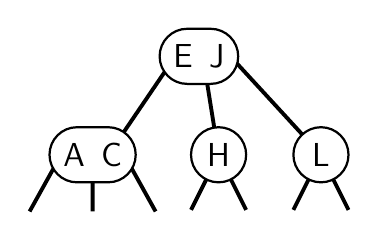
\begin{tikzpicture}[thick,n/.style={draw,fill=white,rectangle,rounded corners=3.5mm,inner xsep=5pt,inner ysep=0pt,minimum height=7mm,minimum width=7mm,font=\large\sffamily}]
\begin{scope}[line width=1.4pt]
\draw (-0.3,0)--(-1.15,-1.25) (0.05,0)--(0.25,-1.25) (0.4,0)--(1.55,-1.25);
\draw (-1.75,-1.25)--++(-0.4,-0.72) (-1.35,-1.25)--++(0,-0.72) (-0.95,-1.25)--++(0.4,-0.72);
\draw (0.25,-1.25)--++(-0.35,-0.7) (0.25,-1.25)--++(0.35,-0.7);
\draw (1.55,-1.25)--++(-0.35,-0.7) (1.55,-1.25)--++(0.35,-0.7);
\end{scope}
\node[n] (r) at (0,0) {E\ \,J};
\node[n] (a) at (-1.35,-1.25) {A\ \,C};
\node[n,circle,inner sep=0pt] (h) at (0.25,-1.25) {H};
\node[n,circle,inner sep=0pt] (l) at (1.55,-1.25) {L};
\end{tikzpicture}
\end{center}
\end{pastexam}

\begin{pastsoln}
本題是 2-3 樹和二元搜尋樹的對應（資結書第~11.1.6~節，那裡寫的是 2-3-4 樹和紅黑樹，2-3 樹是
沒有 4-節點的特例）。 圖裡葉節點下面的短線是空的子樹。

\textbf{a.} 2-節點 $\{x\}$ 就是一個二元節點 $x$。 3-節點 $\{a, b\}$（$a < b$）拆成兩個二元節點，
用一條邊連起來：上面放 $a$、$b$ 當它的右子節點，或上面放 $b$、$a$ 當它的左子節點，兩種都對。
原本的三棵子樹依鍵的範圍接上去：小於 $a$ 的接在 $a$ 的左邊，介於 $a$、$b$ 之間的接在中間
（$a$ 的右邊或 $b$ 的左邊），大於 $b$ 的接在 $b$ 的右邊。 連接 $a$、$b$ 的那條邊就是「3-節點
裡面的邊」，在紅黑樹裡就是連到紅色節點的邊。

這裡兩個 3-節點都取「小的在上面」：$\{E, J\}$ 變成 $E$ 帶右子節點 $J$，$\{A, C\}$ 變成 $A$ 帶右
子節點 $C$。 $H$ 介於 $E$、$J$ 之間，接在 $J$ 的左邊；$L > J$，接在 $J$ 的右邊。 粗線是 3-節點
裡面的邊：

\begin{center}
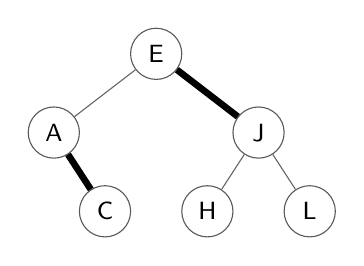
\begin{tikzpicture}[
    btn/.style={circle, draw=black!65, line width=0.4pt, minimum size=6.5mm, inner sep=0pt, font=\small\sffamily},
    level distance=10mm, edge from parent/.style={draw=black!60, thin},
    hl/.style={edge from parent/.style={draw=black, line width=2.4pt}},
    level 1/.style={sibling distance=26mm}, level 2/.style={sibling distance=13mm}]
\node[btn] {E}
    child {node[btn] {A}
        child[missing]
        child[hl] {node[btn] {C}}}
    child[hl] {node[btn] {J}
        child[edge from parent/.style={draw=black!60, thin}] {node[btn] {H}}
        child[edge from parent/.style={draw=black!60, thin}] {node[btn] {L}}};
\end{tikzpicture}
\end{center}
檢查：中序是 $A, C, E, H, J, L$，由小到大，是二元搜尋樹。 粗線兩條：$E$--$J$、$A$--$C$。

如果 3-節點改取「大的在上面」，$\{E, J\}$ 變成 $J$ 帶左子節點 $E$，樹是
$J(E(C(A, \cdot), H), L)$，粗線是 $J$--$E$、$C$--$A$，也是正確答案。 b 的結果會因此不同，下面
兩種都寫。

\textbf{b.} 根有兩個子節點，照二元搜尋樹的刪除（資結書第~9.2~節），用左子樹裡最大的鍵（前驅）
取代根，再把那個鍵從左子樹拿掉。

\textbf{照 a 的畫法。} 根是 $E$，左子樹是 $A(\cdot, C)$，最大的是 $C$。 $C$ 是葉子，直接拿掉，
$C$ 放到根的位置：

\begin{center}
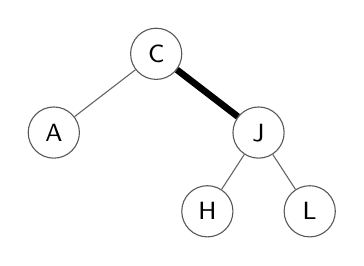
\begin{tikzpicture}[
    btn/.style={circle, draw=black!65, line width=0.4pt, minimum size=6.5mm, inner sep=0pt, font=\small\sffamily},
    level distance=10mm, edge from parent/.style={draw=black!60, thin},
    hl/.style={edge from parent/.style={draw=black, line width=2.4pt}},
    level 1/.style={sibling distance=26mm}, level 2/.style={sibling distance=13mm}]
\node[btn] {C}
    child {node[btn] {A}}
    child[hl] {node[btn] {J}
        child[edge from parent/.style={draw=black!60, thin}] {node[btn] {H}}
        child[edge from parent/.style={draw=black!60, thin}] {node[btn] {L}}};
\end{tikzpicture}
\end{center}
粗線只剩 $C$--$J$。 原本的 3-節點 $\{A, C\}$ 少了 $C$，$A$ 變成 2-節點，$A$--$C$ 那條邊也跟著
沒了；根原本的 3-節點 $\{E, J\}$ 換成 $\{C, J\}$，$J$ 還是根的右子節點，所以 $C$--$J$ 是 3-節點
裡面的邊。 對應的 2-3 樹是根 $\{C, J\}$、三個子節點 $A$、$H$、$L$，所有葉子同一層，仍然是合法
的 2-3 樹：這正是在 2-3 樹裡用前驅刪除 $E$ 的結果（葉子 $\{A, C\}$ 拿走 $C$ 還剩 $A$，不會不足）。

\textbf{照「大的在上面」的畫法。} 根是 $J$，左子樹 $E(C(A, \cdot), H)$ 裡最大的是 $H$。 $H$ 是葉子，
拿掉後放到根，得到 $H(E(C(A, \cdot), \cdot), L)$。 根的 3-節點 $\{E, J\}$ 變成 $\{E, H\}$，粗線是
$H$--$E$ 和 $C$--$A$。 但這時 $E$ 的右子樹是空的：2-3 樹的根 $\{E, H\}$ 中間那個子節點不見了，
葉子不在同一層，已經不是合法的 2-3 樹。 要修，就照 2-3 樹的刪除向左兄弟 $\{A, C\}$ 借一個鍵
（資結書第~11.1.4~節）：$E$ 下來、$C$ 上去，2-3 樹變成根 $\{C, H\}$、子節點 $A$、$E$、$L$，二元
樹是 $H(C(A, E), L)$，粗線 $H$--$C$。 題目只要求換掉根並標出 3-節點的邊，寫到
$H(E(C(A, \cdot), \cdot), L)$ 並說明它需要再調整即可。
\end{pastsoln}
